\chapter{Estado da Arte}
\label{chap:estadodaarte}

Esta secção tem como objetivo apresentar o estado da arte, analisando um conjunto de ferramentas e/ou produtos que partilham funcionalidades, ou que assentam em modelos de negócio semelhantes ao \textit{Blended4Future}. Em particular, privilegia-se a exploração de plataformas digitais concebidas para a divulgação, gestão e acompanhamento de projetos ou estágios de carácter internacional, onde a colaboração entre instituições, empresas e estudantes assume um papel central.

Para além de identificar soluções com finalidades comparáveis, pretende-se também realçar as suas principais características distintivas, apontando os pontos fortes, limitações e contextos de utilização.

\section{Contexto}

As ferramentas de procura de estágios \textit{online} direcionadas para estudantes Erasmus desempenham um papel central na mobilidade académica e profissional dentro do espaço europeu. Estas plataformas surgem como mediadoras entre estudantes que procuram uma experiência internacional de trabalho e organizações que disponibilizam oportunidades de estágio, funcionando como pontos de encontro digitais que facilitam a divulgação, a pesquisa e a seleção de estágios.

A sua principal vantagem reside na capacidade de centralizar num único espaço inúmeras ofertas provenientes de diferentes países, permitindo ao estudante filtrar as oportunidades de acordo com critérios como a área de estudo, a duração do estágio, o país de destino ou o tipo de instituição de acolhimento. Este mecanismo é particularmente relevante no contexto do programa Erasmus+, uma vez que os estudantes têm frequentemente requisitos específicos a cumprir, quer em termos académicos (reconhecimento de créditos ECTS), quer em termos de apoio logístico (alojamento, bolsas ou compatibilidade com calendários universitários).

É importante compreender que o \textit{website} do \textit{Blended4Future} tem como principal função a apresentação dos projetos que foram ou que se encontram em desenvolvimento no âmbito do programa. Por sua vez, as plataformas analisadas neste estado da arte centram-se sobretudo na oferta de estágios internacionais. Apesar desta diferença de enfoque, a análise destas ferramentas revela-se pertinente, uma vez que partilham um modelo de negócio semelhante, baseado na interligação entre estudantes, instituições de ensino e empresas, visando a promoção de oportunidades de desenvolvimento académico e profissional em contexto internacional.

\section{ESN - \textit{European Student Network}}

A Erasmus Student Network (ESN) é uma organização sem fins lucrativos fundada em 1989 e atualmente presente em mais de 40 países europeus. O seu objetivo principal é apoiar e enriquecer a experiência de estudantes em mobilidade internacional, nomeadamente no âmbito do programa Erasmus+, mas também de outros programas de intercâmbio académico e profissional. Através de uma vasta rede de secções locais, a ESN promove atividades culturais, sociais e profissionais que favorecem a integração dos estudantes nos países de acolhimento.

Para além das suas atividades presenciais, a ESN tem desenvolvido várias plataformas digitais que servem de apoio à comunidade estudantil, oferecendo acesso a informações sobre oportunidades de estágio, bolsas de estudo, e até serviços de voluntariado internacional. Estas ferramentas constituem um importante meio de ligação entre estudantes, instituições e empresas, permitindo assim fomentar uma experiência de mobilidade mais completa e enriquecedora.

\subsection{erasmusintern.org}

Dentro da ampla rede de iniciativas desenvolvidas pela Erasmus Student Network (ESN), destaca-se particularmente o projeto \textit{ErasmusIntern.org}, que constitui o departamento dedicado à divulgação de oportunidades de estágio em formato online.

\begin{figure}[h!tbp]
    \centering
    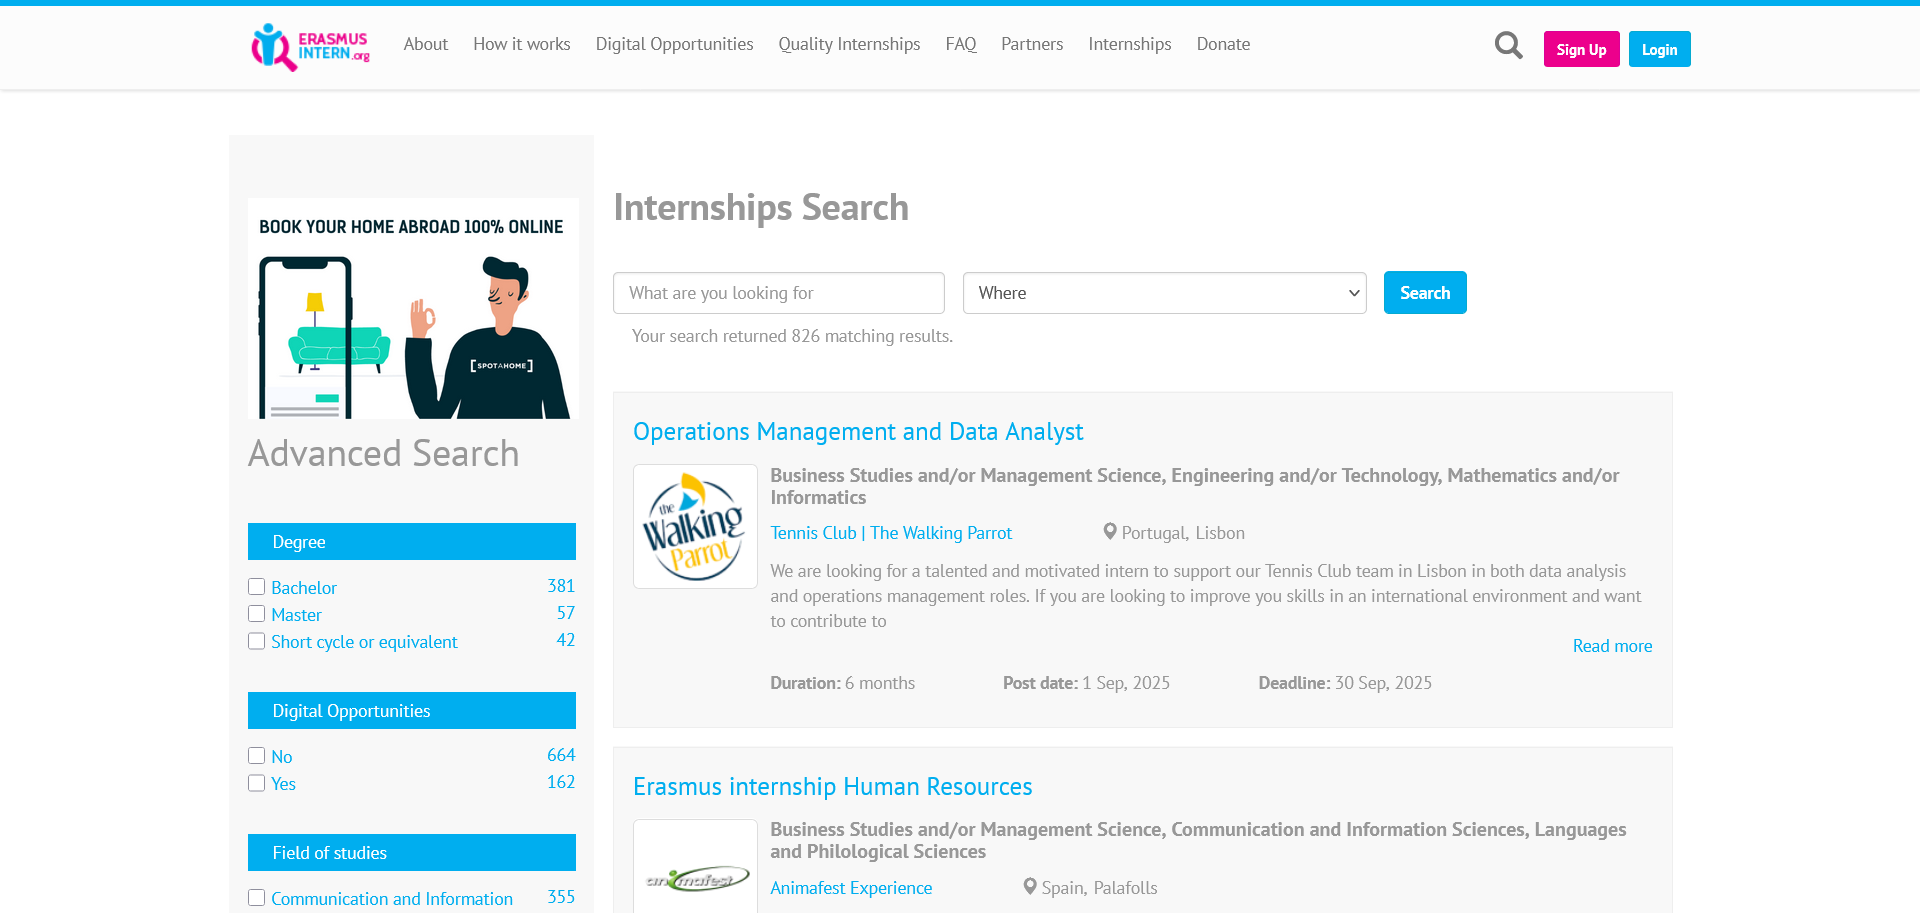
\includegraphics[width=0.7\linewidth]{capitulos/cap2-estadodaarte/assets/image/esn/internship-org.png}
    \caption{\textit{Website} do erasmusintern.org}
    \label{fig:erasmus-intern-homepage}
\end{figure}

Num contexto desta natureza, em que a diversidade académica e cultural dos utilizadores é extremamente elevada, a disponibilização de mecanismos de pesquisa eficazes assume um papel central. A existência de filtros específicos, nomeadamente por área de estudo, setor de atividade, localização geográfica ou duração do estágio, torna-se fundamental para garantir que os estudantes encontram rapidamente as oportunidades que melhor correspondem ao seu perfil e às suas expectativas.

A plataforma \textit{ErasmusIntern.org} destaca-se pela abrangência, oferecendo oportunidades em diversas áreas de estudo e permitindo ao utilizador recorrer a um vasto conjunto de filtros de pesquisa para personalizar a sua procura (ver Figura \ref{fig:erasmus-intern-filters}).

Em contraste, o \textit{Blended4Future} adota uma abordagem mais focada, centrando-se sobretudo em três áreas específicas: Informática, Marketing e Design. Ao invés de promover uma dispersão de oportunidades, o projeto visa potenciar a interdisciplinaridade entre estas áreas, reunindo estudantes de diferentes especializações num mesmo contexto de colaboração. Esta estratégia procura não apenas responder às necessidades de mercado nestes domínios, mas também tende a refletir projetos reais e a treinar os estudantes para um mercado de trabalho exigente, proporcionando-lhes a oportunidade de colaborar diretamente com empresas parceiras.

\begin{figure}[h!tbp]
    \centering
    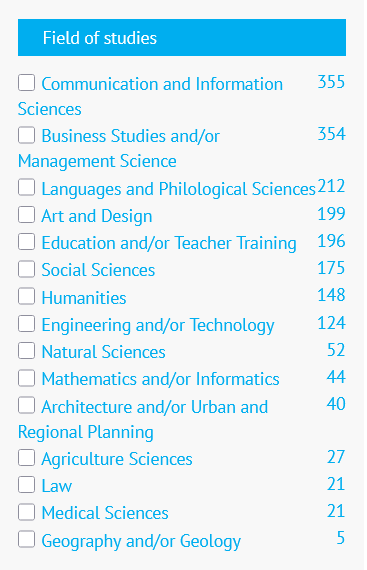
\includegraphics[width=0.3\linewidth]{capitulos/cap2-estadodaarte/assets/image/esn/erasmus-intern filters.png}
    \caption{Filtros de pesquisa divididos por \textit{Area de Estudo} do erasmusintern.org}
    \label{fig:erasmus-intern-filters}
\end{figure}

\section{PRAXIS}

A PRAXIS uma função bastante semelhante à desempenhada pela \textit{ErasmusIntern.org}, centrando-se igualmente na promoção e intermediação de estágios internacionais para estudantes universitários. A PRAXIS Network resulta de uma colaboração entre diversas instituições de ensino superior europeias, procurando criar uma rede sólida que facilite a mobilidade estudantil e, simultaneamente, aumente a cooperação entre universidades e entidades empregadoras. 

Na página inicial da plataforma PRAXIS evidencia-se, desde logo, a centralidade atribuída aos dois atores fundamentais deste tipo de iniciativa: os estudantes, enquanto beneficiários diretos das oportunidades de estágio, e as empresas, que se apresentam como entidades promotoras. Esta lógica de funcionamento assenta na criação de um ponto de encontro entre oferta e procura, permitindo um processo de intermediação simples e acessível.

De forma semelhante, o Blended4Future identifica como público-alvo tanto os estudantes como as empresas, reconhecendo, no entanto, um terceiro interveniente igualmente relevante: as universidades. A inclusão das instituições de ensino superior representa um diferencial importante, uma vez que estas desempenham um papel central na mediação académica e na validação das experiências desenvolvidas. Para além de atuar como intermediário entre alunos e organizações, o projeto procura também atrair um número crescente de universidades parceiras, reforçando a credibilidade da plataforma e ampliando o alcance das oportunidades disponibilizadas.

\begin{figure}[h!tbp]
    \centering
    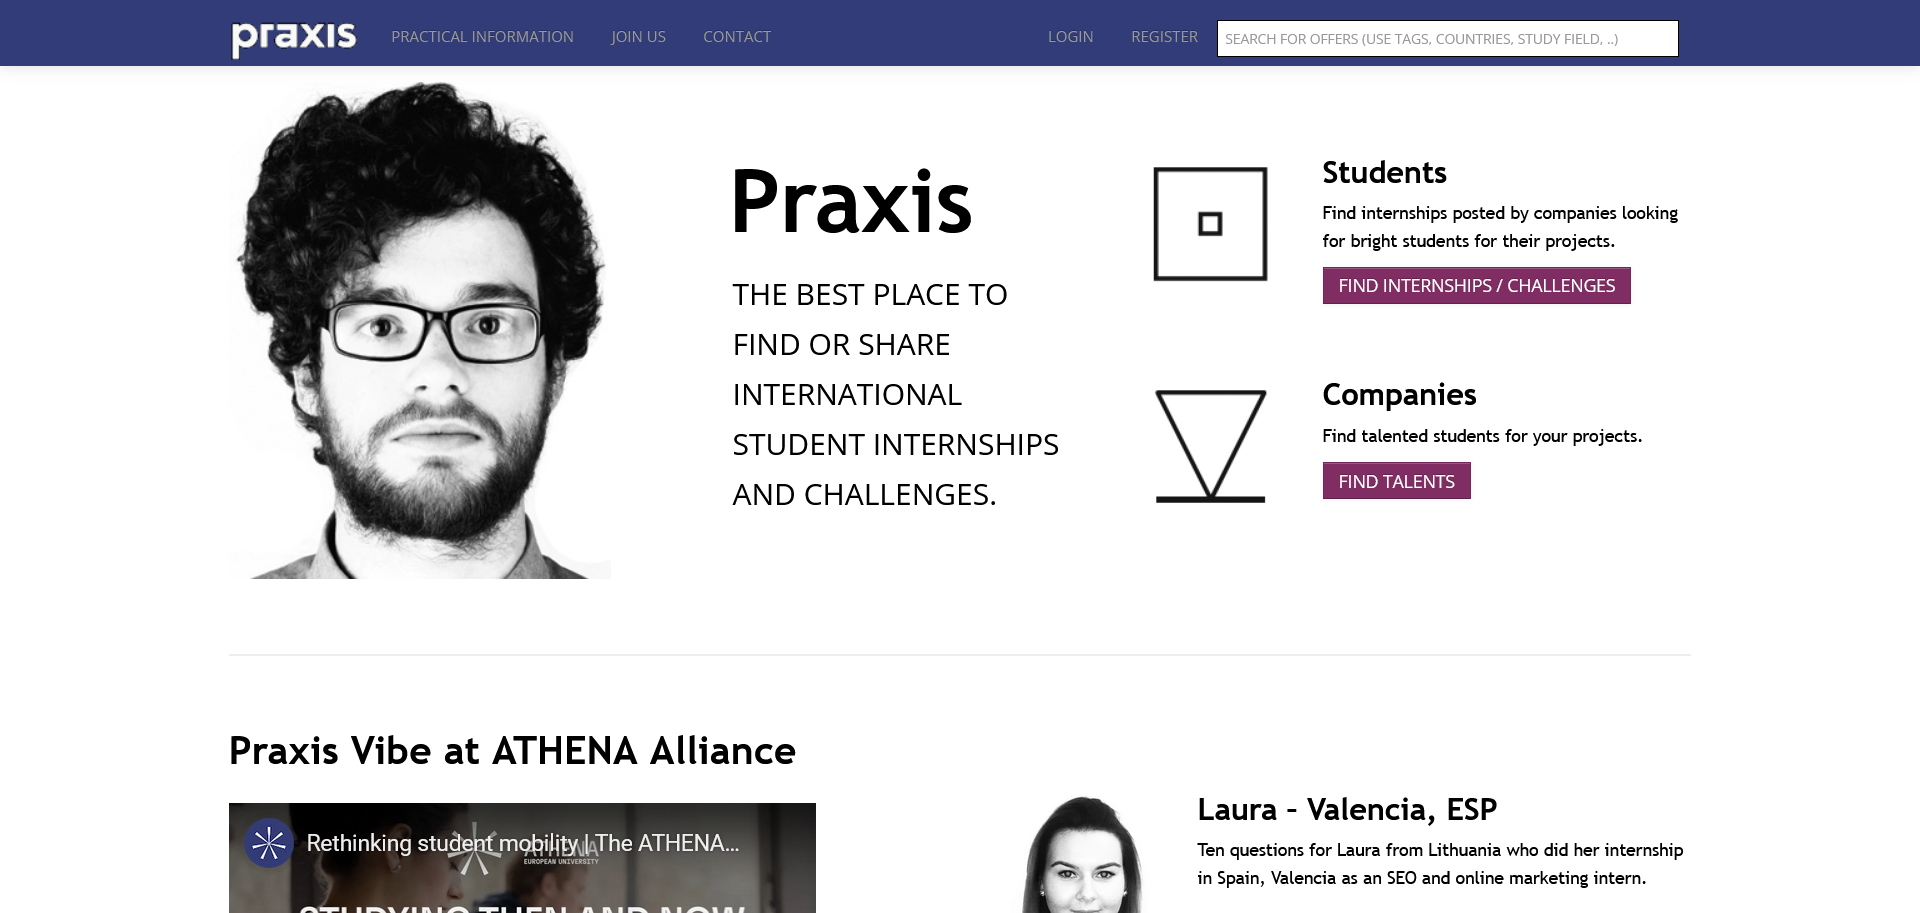
\includegraphics[width=0.9\linewidth]{capitulos/cap2-estadodaarte/assets/image/praxis/praxis-homepage.png}
    \caption{\textit{Home page} da praxisnetwork.eu}
    \label{fig:praxis-homepage}
\end{figure}


\begin{figure}[h!tbp]
    \centering
    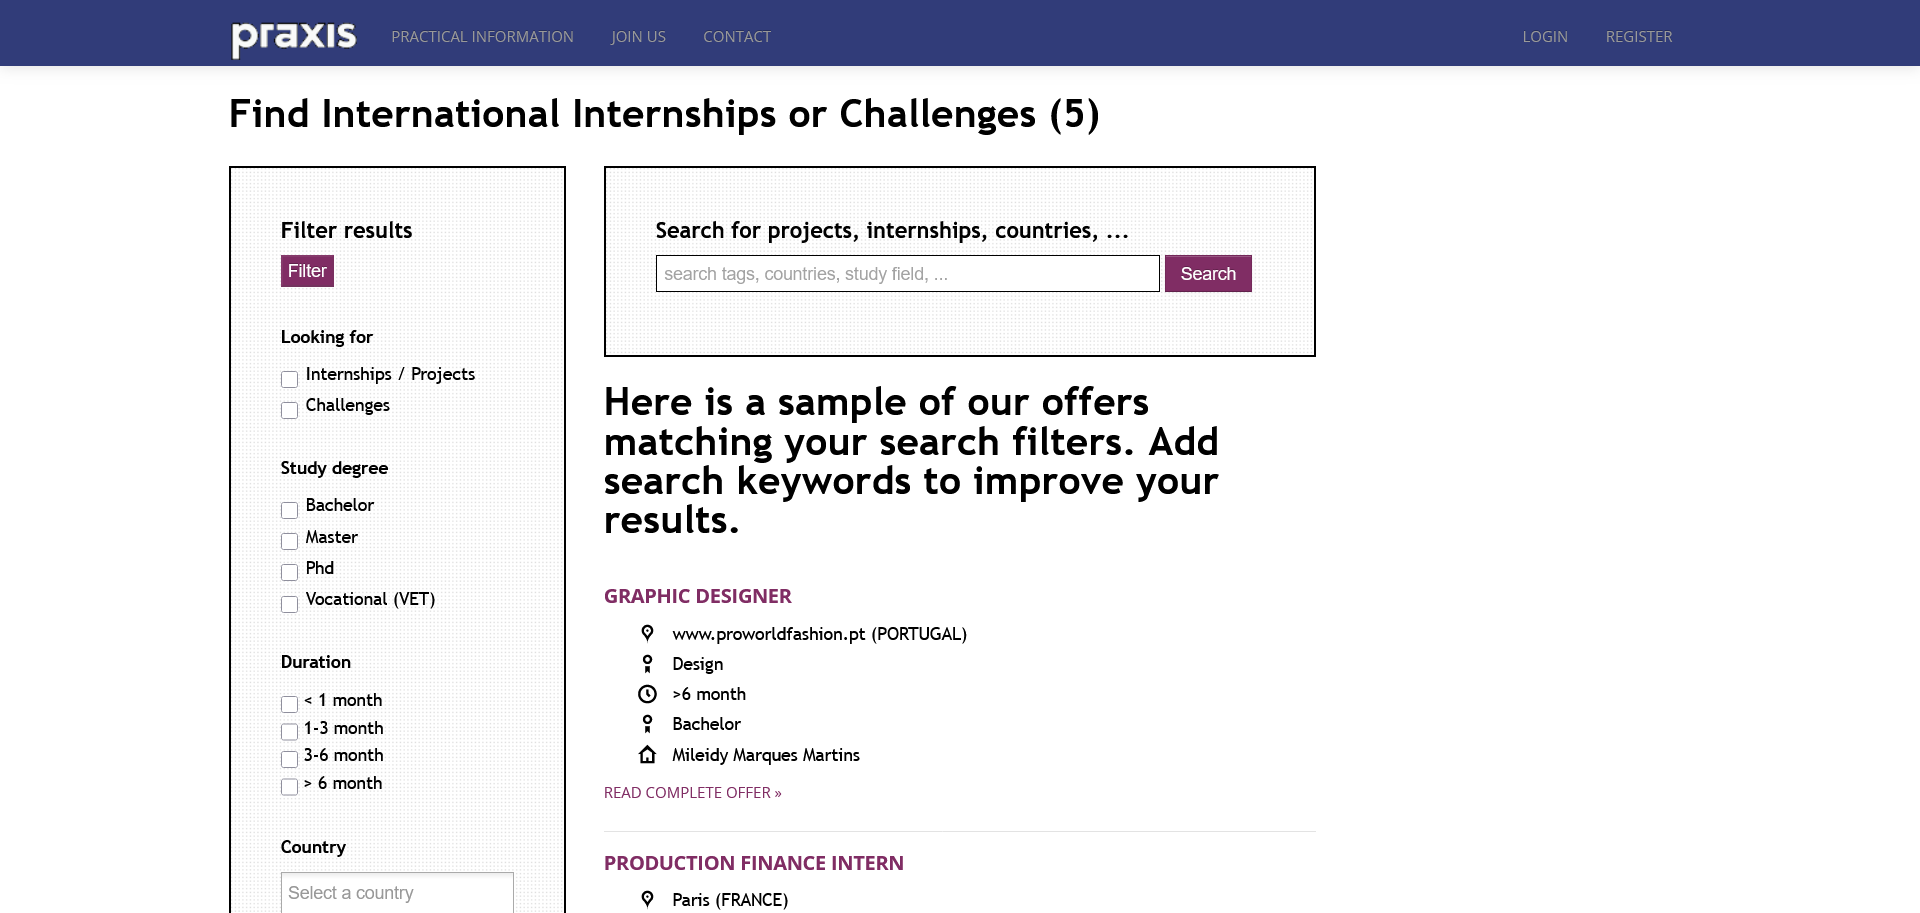
\includegraphics[width=0.9\linewidth]{capitulos/cap2-estadodaarte/assets/image/praxis/praxis-search.png}
    \caption{Página de pesquisa da PRAXIS}
\end{figure}

\section{\textit{Spain Internship}}

A \textit{Spain Internship} é uma organização dedicada à oferta de estágios internacionais, com enfoque particular no território espanhol, mas aberta a candidatos de toda a Europa. Tal como as referidas anteriormente, esta plataforma funciona como mediadora entre estudantes e empresas, fornecendo serviços de recrutamento, acompanhamento e suporte administrativo, sendo frequentemente utilizada por estudantes em programas de mobilidade europeia.

\begin{figure}[h!tbp]
    \centering
    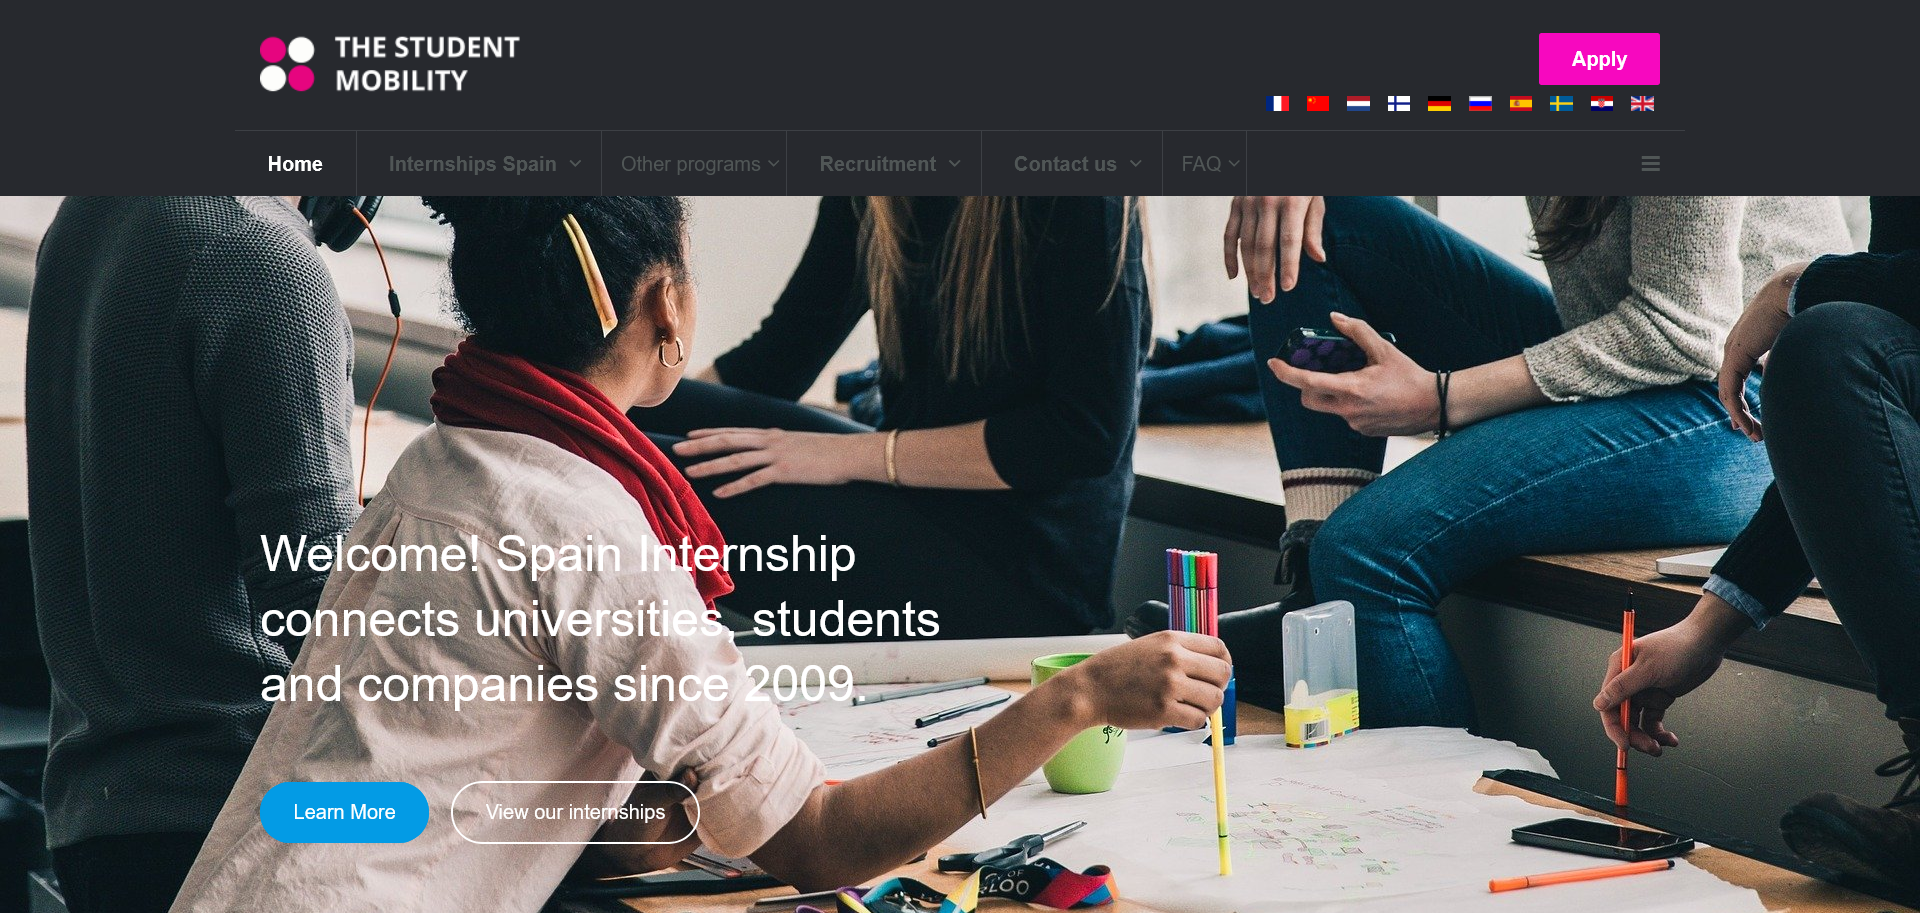
\includegraphics[width=0.9\linewidth]{capitulos/cap2-estadodaarte/assets/image/spain-internship/spain-internship-homepage.png}
    \caption{\textit{Home Page} da \textit{Spain Internship}}
    \label{fig:spain-homepage}
\end{figure}

Mais uma vez, observa-se um forte investimento em ferramentas de filtragem, concebidas para tornar a pesquisa de oportunidades o mais simples e direcionada possível. Paralelamente, estas plataformas disponibilizam mecanismos de contacto direto que facilitam a comunicação entre os três principais atores do ecossistema — estudantes, empresas e universidades —, precisamente os mesmos que constituem o núcleo do modelo de negócio do Blended4Future, como referido anteriormente.

\begin{figure}[h!tbp]
    \centering
    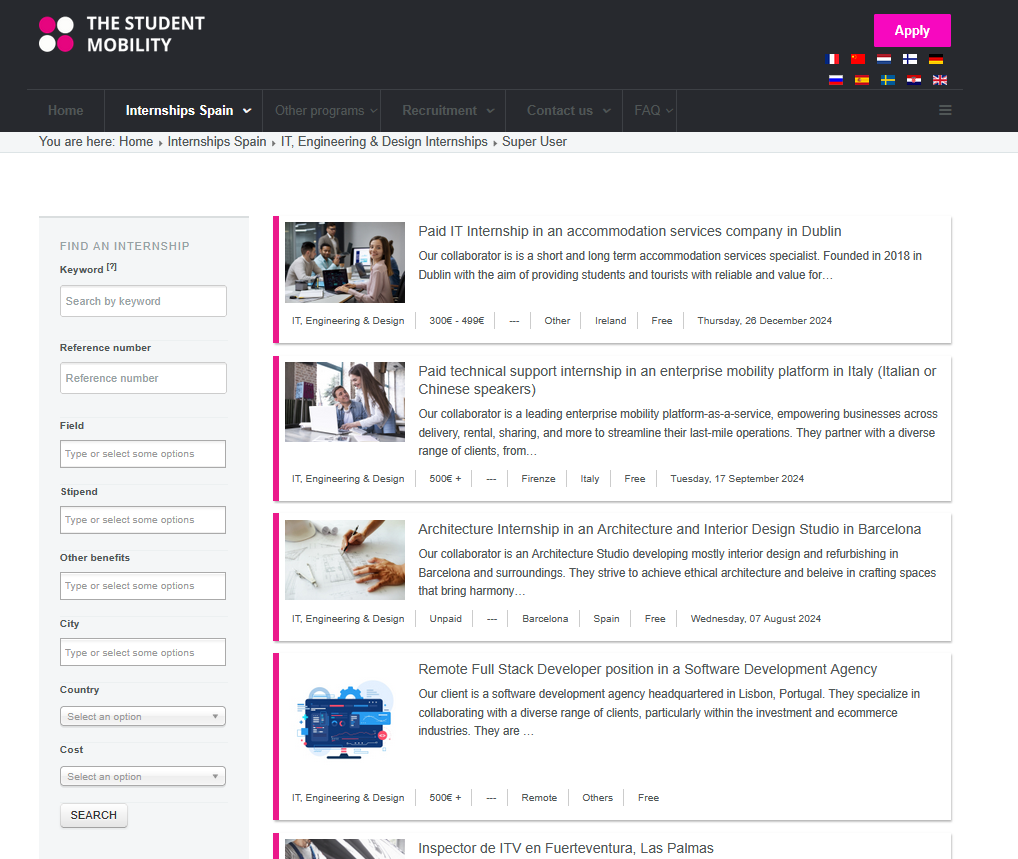
\includegraphics[width=0.9\linewidth]{capitulos/cap2-estadodaarte/assets/image/spain-internship/spain-search.png}
    \caption{Página de pesquisa da \textit{Spain Internship}}
    \label{fig:spain-search}
\end{figure}

\begin{figure}[h!tbp]
    \centering
    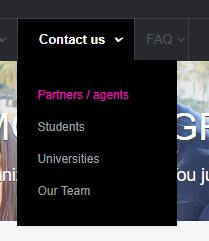
\includegraphics[width=0.3\linewidth]{capitulos/cap2-estadodaarte/assets/image/spain-internship/spain-contact-list.png}
    \caption{\textit{Dropdown list} para as paginas de contacto}
    \label{fig:spain-contact-list}
\end{figure}

\begin{figure}[h!tbp]
    \centering
    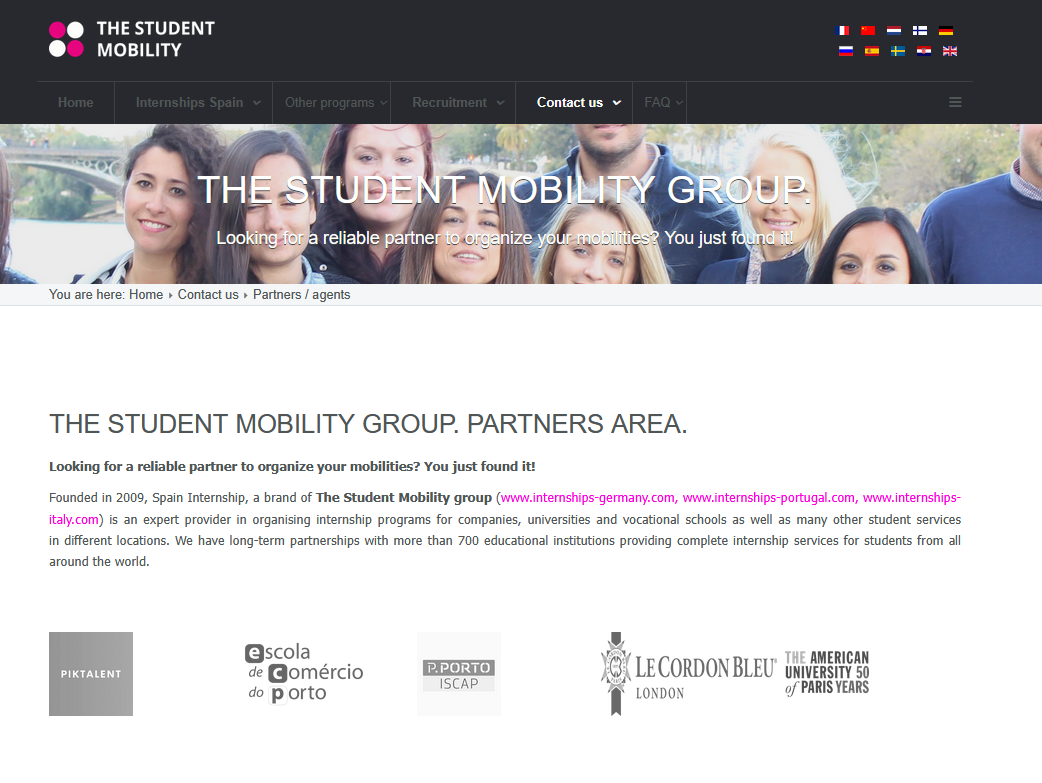
\includegraphics[width=0.7\linewidth]{capitulos/cap2-estadodaarte/assets/image/spain-internship/spain-contact-partners.png}
    \caption{Página de contacto de \textit{partners}}
    \label{fig:spain-contact-partners}
\end{figure}